\subsection{Index comparation}\label{subsec:index-comparation}

So, I've investigated 2 types of indexes \textbf{B-tree} and \textbf{hash}.
I don't investigate 2 other indexes \textbf{GIN} and \textbf{GIST}, because they are not supporting a
\texttt{character varying}, that is actully 95\% of my indexes, so data for the investigation won't be accurate
in that case.

\subsubsection{Size of indexes}

Query that I used to measure indexes size:

\texttt{select pg\_size\_pretty(pg\_relation\_size('index\_ticket\_event\_id')) as index\_ticket\_event\_id,\\
pg\_size\_pretty(pg\_relation\_size('index\_ticket\_user\_id')) as index\_ticket\_user\_id,\\
pg\_size\_pretty(pg\_relation\_size('index\_ticket\_category')) as index\_ticket\_category,\\
pg\_size\_pretty(pg\_relation\_size('index\_event\_date')) as index\_event\_date,\\
pg\_size\_pretty(pg\_relation\_size('index\_event\_title')) as index\_event\_title,\\
pg\_size\_pretty(pg\_relation\_size('index\_user\_email')) as index\_user\_email,\\
pg\_size\_pretty(pg\_relation\_size('index\_user\_name')) as index\_user\_name \\
}

\begin{figure}[h]
    \centering
    \label{fig:hash_index_size}
    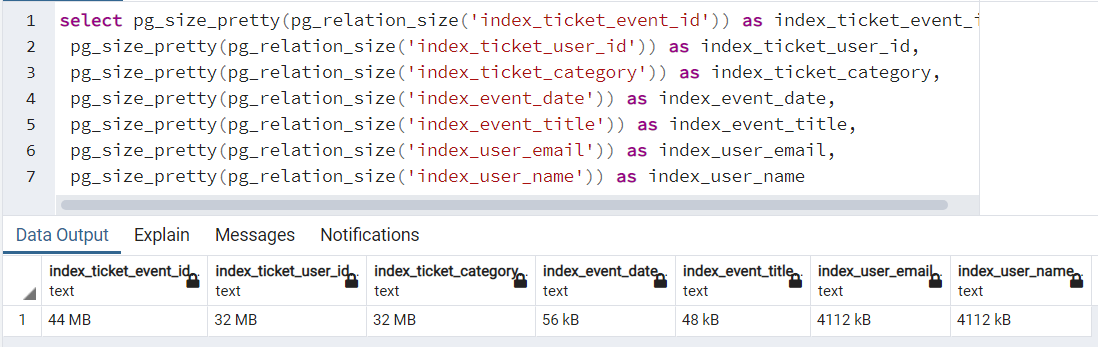
\includegraphics[width=1\textwidth]{images/index_size_hash}
    \caption{Represents how much size each index takes using hash indexes}
\end{figure}

\begin{figure}[h]
    \centering
    \label{fig:b_tree_index_size}
    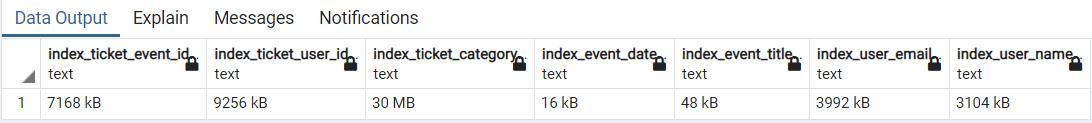
\includegraphics[width=1\textwidth]{images/index_size_b_tree}
    \caption{Represents how much size each index takes using B-tree indexes}
\end{figure}

\subsubsection{Speed of queries}

Query for selecting user by name (exact match):

\texttt{SELECT * FROM public."user" WHERE "name" LIKE 'name 1050'}

\begin{center}
    \begin{tabular}{ | c | c |}
        \hline
        B-tree   & 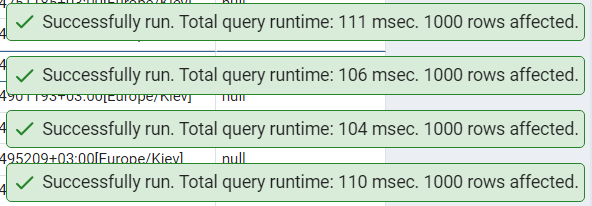
\includegraphics[width=0.8\textwidth]{images/query_select_user_by_email_like_performance_b_tree}   \\ \hline
        hash     & 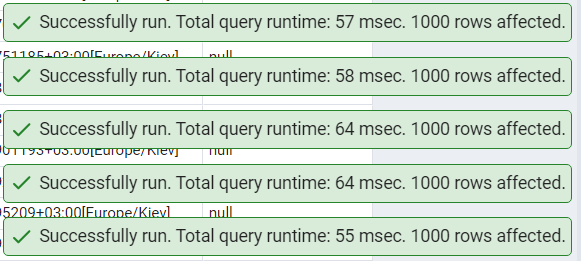
\includegraphics[width=0.8\textwidth]{images/query_select_user_by_email_like_performance_hash}     \\ \hline
        no index & 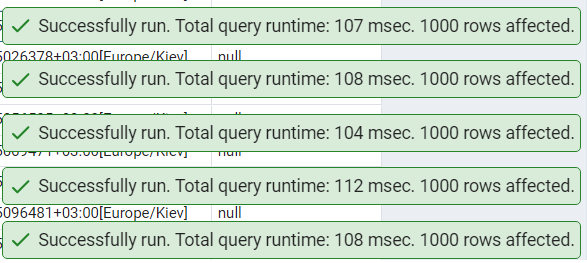
\includegraphics[width=0.8\textwidth]{images/query_select_user_by_email_like_performance_no_index} \\ \hline
    \end{tabular}
\end{center}

\newpage
Query for selecting user by name (contains):

\texttt{SELECT * FROM public."user" WHERE name LIKE "\%name 5\%"}

\begin{center}
    \begin{tabular}{ | c | c |}
        \hline
        B-tree   & 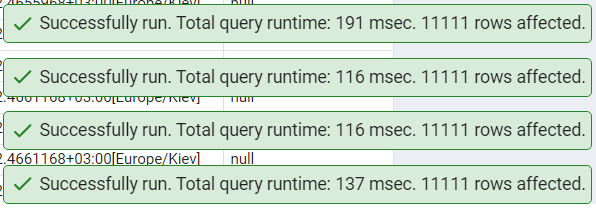
\includegraphics[width=0.8\textwidth]{images/query_select_user_by_name_like_performance_b_tree}   \\ \hline
        hash     & 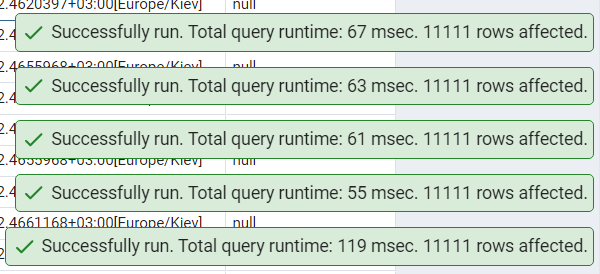
\includegraphics[width=0.8\textwidth]{images/query_select_user_by_name_like_performance_hash}     \\ \hline
        no index & 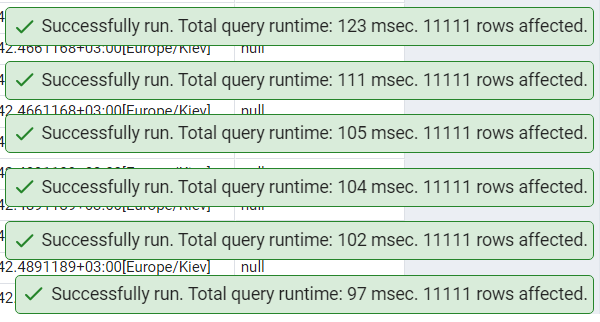
\includegraphics[width=0.8\textwidth]{images/query_select_user_by_name_like_performance_no_index} \\ \hline
    \end{tabular}
\end{center}

\newpage
Query for selecting user by email (contains):

\texttt{SELECT * FROM public."user" WHERE email LIKE "\%17@\%"}

\begin{center}
    \begin{tabular}{ | c | c |}
        \hline
        B-tree   & 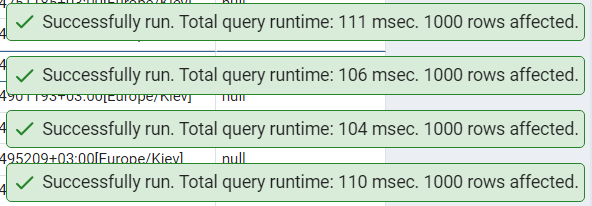
\includegraphics[width=0.8\textwidth]{images/query_select_user_by_email_like_performance_b_tree}   \\ \hline
        hash     & 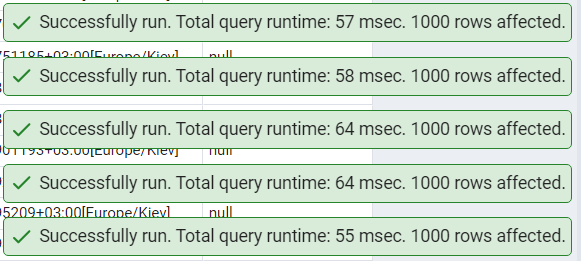
\includegraphics[width=0.8\textwidth]{images/query_select_user_by_email_like_performance_hash}     \\ \hline
        no index & 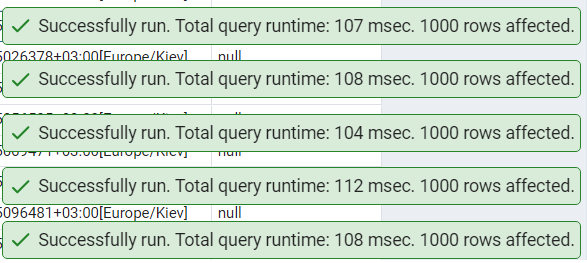
\includegraphics[width=0.8\textwidth]{images/query_select_user_by_email_like_performance_no_index} \\ \hline
    \end{tabular}
\end{center}

\newpage
Query by email from users that have at least one ticket (contains):

\texttt{
    SELECT public."user".* FROM public."user" \\
    WHERE (SELECT COUNT(*)FROM public.ticket WHERE public.ticket.id = public."user".id) > 0 \\
    AND public."user".email LIKE "\%77@\%" \\
}

\begin{center}
    \begin{tabular}{ | c | c |}
        \hline
        B-tree   & 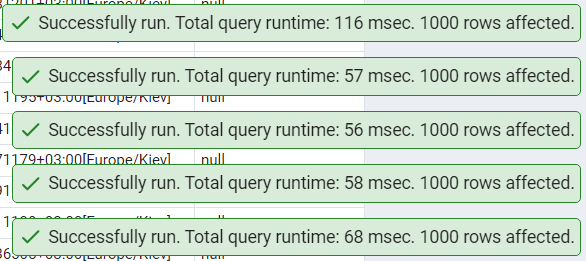
\includegraphics[width=0.8\textwidth]{images/query_select_user_with_tickets_by_email_like_performance_b_tree}   \\ \hline
        hash     & 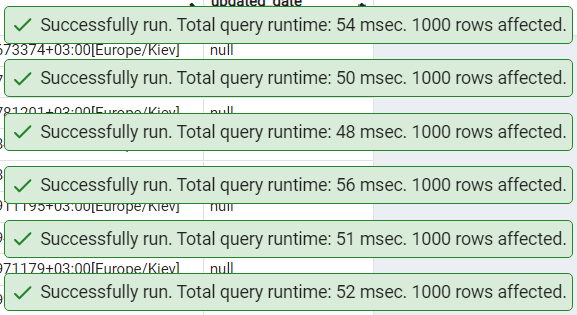
\includegraphics[width=0.8\textwidth]{images/query_select_user_with_tickets_by_email_like_performance_hash}     \\ \hline
        no index & 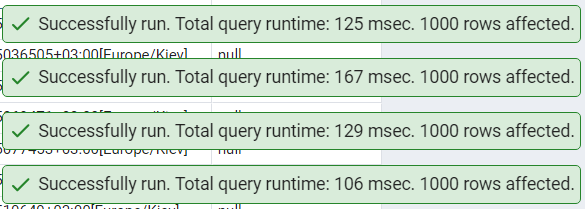
\includegraphics[width=0.8\textwidth]{images/query_select_user_with_tickets_by_email_like_performance_no_index} \\ \hline
    \end{tabular}
\end{center}

\subsection{My conclusion}\label{subsec:my-conclusion}

So as I can see \textbf{B-tree} index is not very useful in my case, I guess it's because
my indexes are almost refers \texttt{character varying} types and that's why \textbf{B-tree} is
not very efficient.

Taking look on the size which indexes are taking, \textbf{hash} is on the figure and on the \textbf{b-tree} figure,
\textbf{hash} index takes more size than \textbf{b-tree}, but taking a look at the efficient comparing tables
\textbf{hash} is more-more efficient in case of \texttt{character varying} indexes.
